\chapter{Background}
Some text

\section{Biology}

\begin{figure}[h]
    \centering
    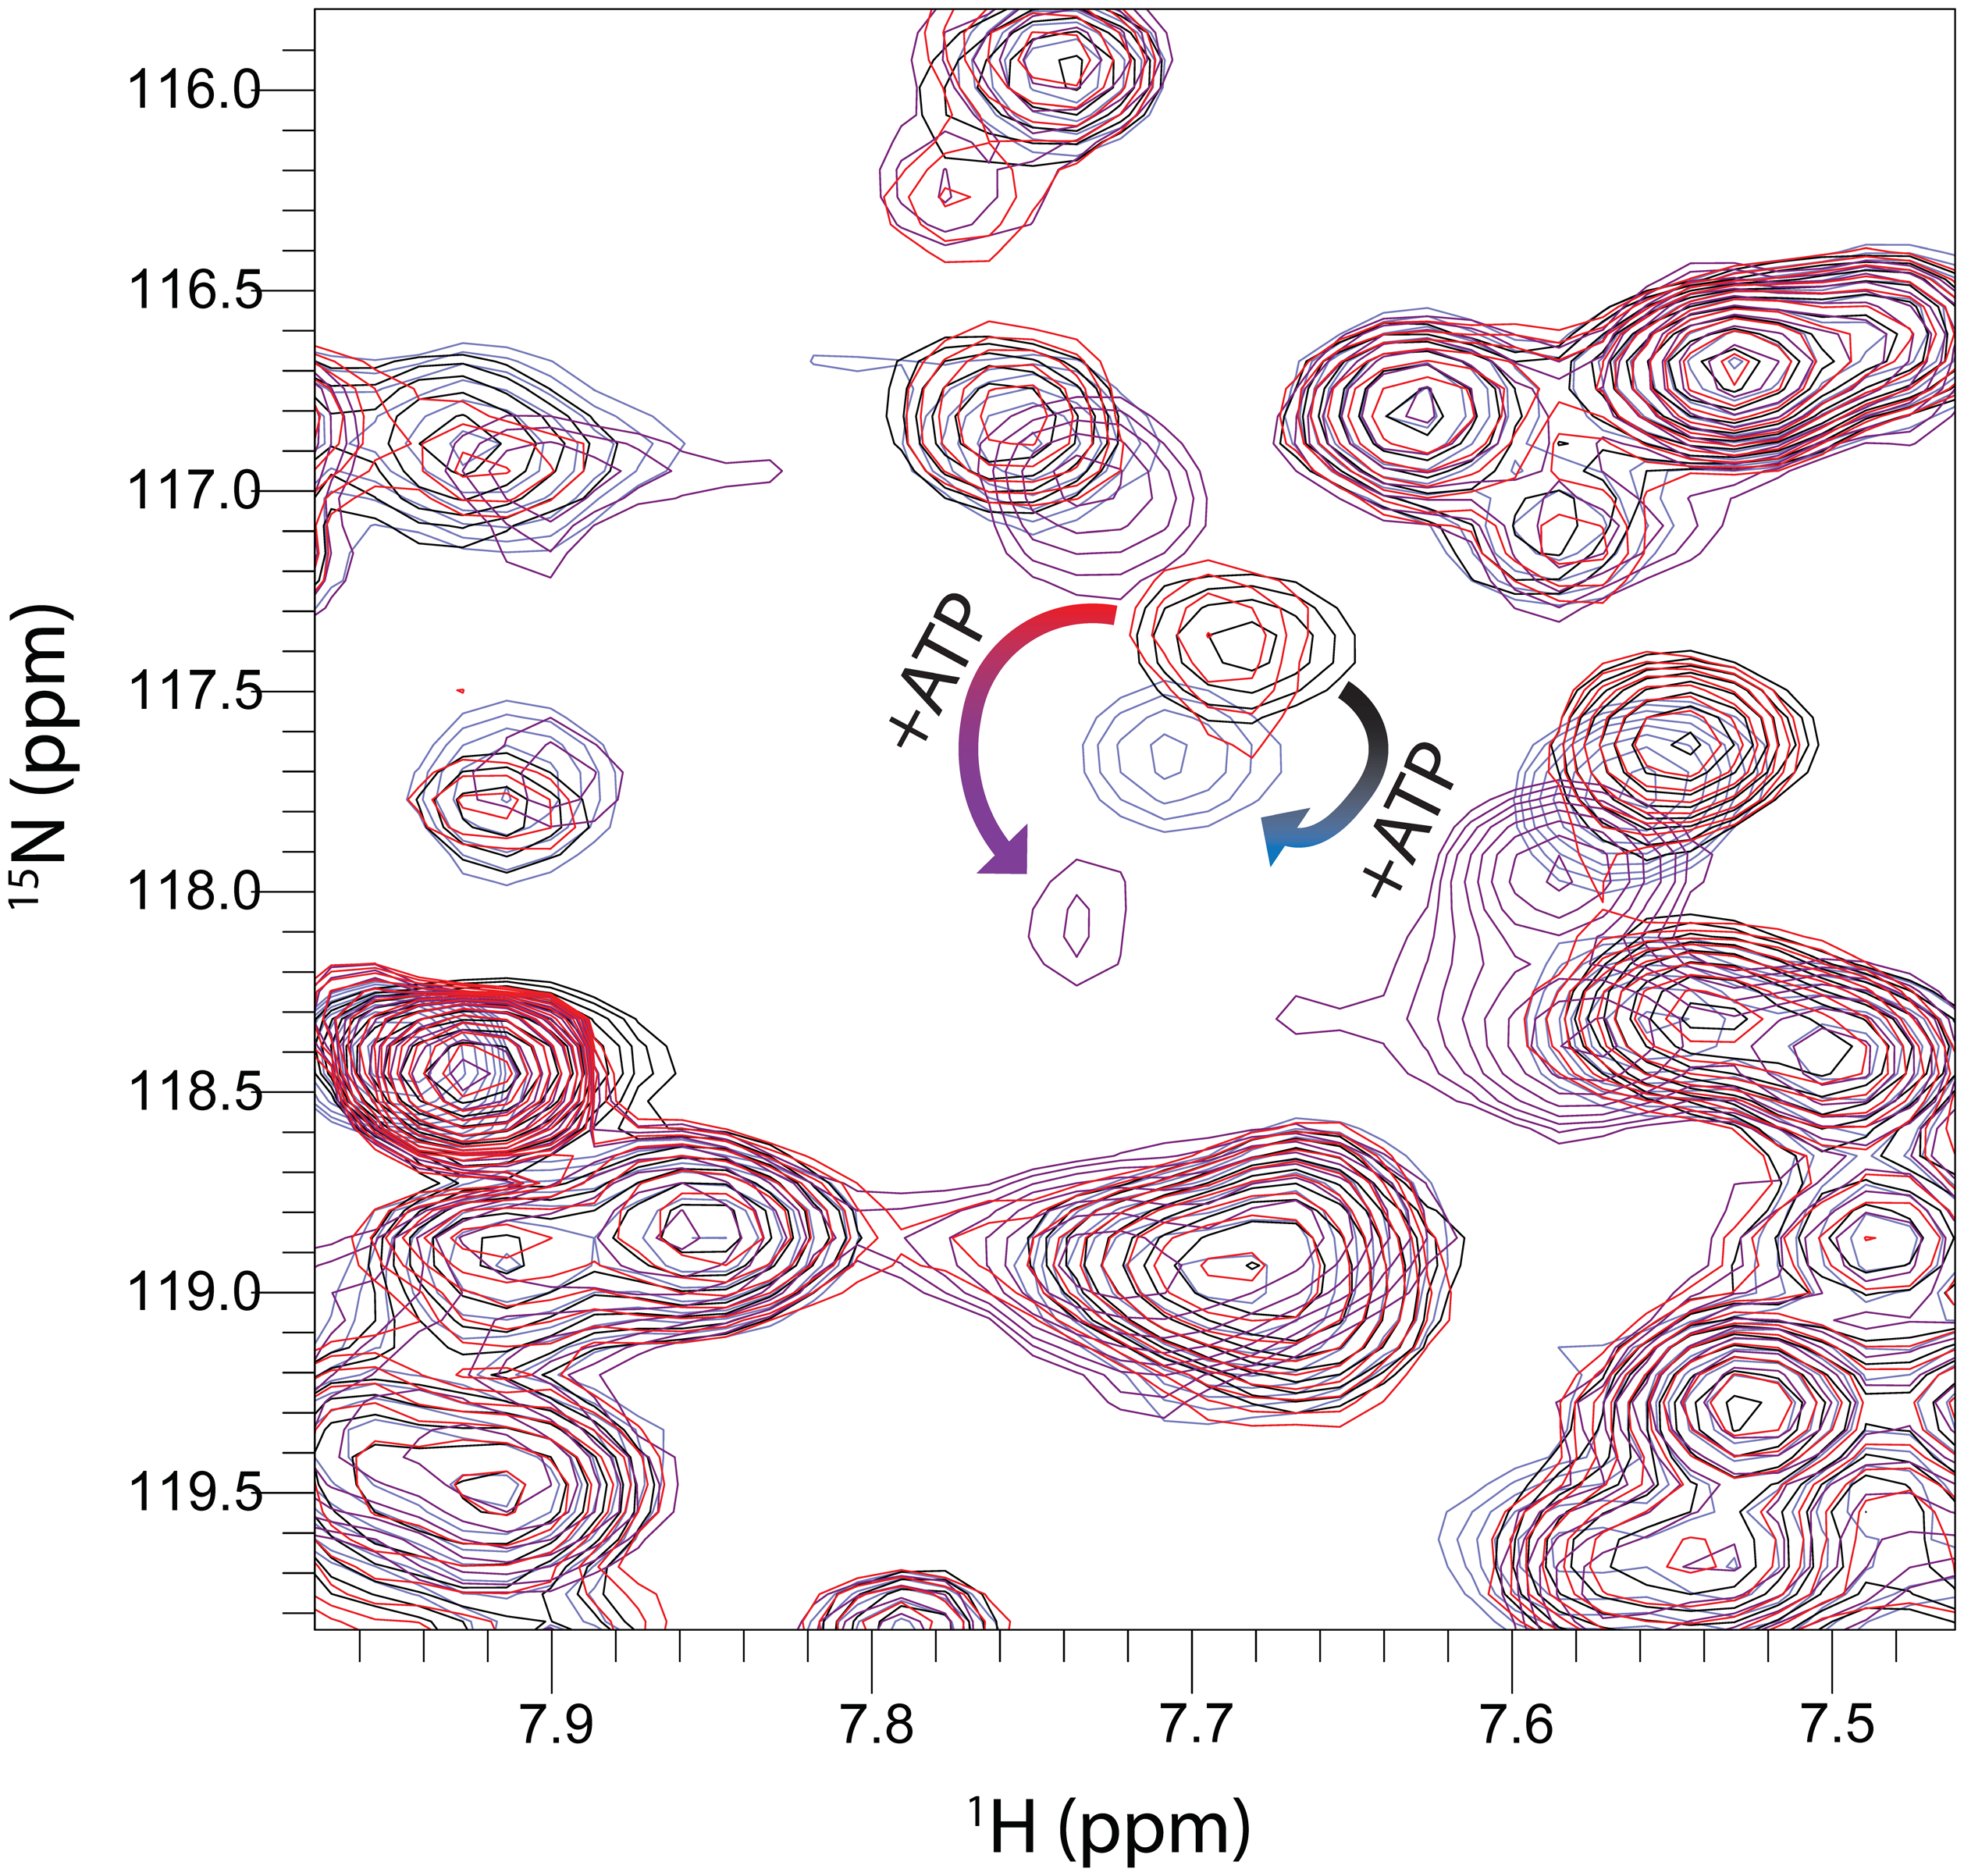
\includegraphics[width=0.75\textwidth]{fig_01.png}
    \caption{What a cool image.}
    \label{fig:f01}
\end{figure}

\newpage
\section{Chemistry}

\newpage
\section{Maths}

Oh well, let's do some maths! \\

$f(x)=x^2$

\begin{equation}
		(x+y)^3 = (x+y)(x+y)^2
       		    =(x+y)(x^2+2xy+y^2)
                =x^3+3x^2y+3xy^3+x^3
\end{equation}

\begin{equation}
	\begin{split}
		(x+y)^3&=(x+y)(x+y)^2 \\
       		   &=(x+y)(x^2+2xy+y^2) \\
               &=x^3+3x^2y+3xy^3+x^3
	\end{split}
    \label{useful_name}
\end{equation}

\newpage
\section{Computer Science}

\subsection{Bioinformatics}

\begin{table}[h]
 \caption{Atom groups used for CVs in alternate string method algorithm.}\vspace{0.5cm}
 \centering
	\begin{tabular}{|c| c| c|}
	\hline
	& \textbf{Group1} & \textbf{Group2} \\
	\hline
	1 & Asn549:N$\delta$2 & Glu565:C$\delta$ \\
	\hline
	2 & Asn549:N$\delta$2 & $\alpha$ carbons of $\alpha$C helix residues (526-541) \\
	\hline
	3 & pTyr657:P & Arg649:C$\zeta$ \\
	\hline
	\end{tabular}
\end{table}
